% Nome do capítulo
\chapter{METODOLOGIA}
% Label para referenciar
\label{cap3}

% Diminuir espaçamento entre título e texto
\vspace{-1.9cm}

% Texto do capítulo

Este capítulo descreve a metodologia construída para o desenvolvimento do aplicativo, apresentando o levantamento de requisitos, prototipação, plano de testes elaborado e homologação.

    \section{Levantamento de Requisitos}

    Para que o desenvolvimento do trabalho esteja alinhado as necessidades do laboratório de audiovisual e fotografia seria preciso, em um primeiro momento, elicitar todos os requisitos arquiteturais (funcionais e não funcionais) de maneira que o entedimento do escopo do projeto fique claro e atenda o objetivo principal que é contribuir na gestão de empréstimos de equipamentos do laboratório. Os requisitos são descritos textualmente para identificar as funcionalidades e características que a aplicação deve possuir para conseguir realizar as ações que, em conjunto, solucionam o problema exposto, sendo assim, tem-se uma visão de alto nível do projeto, o que torna sua interpretação fácil a todos os envolvidos. 
    
    Conforme o problema exposto, o aplicativo \textit{mobile} funcionará como um gestor de empréstimos dos equipamentos do laboratório, no perfil de "administrador" que será atribuído aos monitores e técnicos do laboratório será possível cadastrar novos equipamentos além de consultar/aprovar/reprovar todas as solicitações de empréstimo feitas por alunos, enquanto que o alunos poderão consultar todos os artefatos disponíveis, solicitá los via plataforma e atentar se sobre os prazos de devolução por meio de alertas e notificações emitidas.
    
    \subsection{Entrevistas}
    
    Foi realizada uma entrevista com o profissional técnico responsável pelo laboratório de audiovisual da PUC Minas Unidade São Gabriel, para validar os requisitos da aplicação e concretizar o entendimento do problema que este trabalho propõe a resolver.
    
    Como metodologia, foi utilizado uma entrevista não estruturada, em que não houve a criação de um roteiro prévio, mas com perguntas bem objetivas sobre o problema em geral enquanto que o entrevistador teve a liberdade de se aprofundar em determinados tópicos que julgasse relevantes para o contexto. Durante a entrevista foram abordados os seguintes tópicos:
     
    1. \textbf{Como é o atual processo de empréstimos dos equipamentos:} foco em entender o contexto de ponta a ponta e como é feito a gestão/controle dos equipamentos e suas devoluções.
    
    2. \textbf{Se existe a necessidade de informatizar o processo de empréstimos:} questões com o objetivo de identificar se a solução proposta seria efetivamente utilizada para atender as necessidades de negócio do laboratório.
    
    O entrevistado validou a utilidade e importância do aplicativo para a gestão de empréstimo dos equipamentos, enfatizando a relevância de informatizar esse processo interno na Universidade. Para os monitores e técnicos, seria muito satisfatório realizar estes procedimentos, atualmente manuais, de maneira informatizada e ágil. Durante a entrevista, foi afirmado que é essencial que o aplicativo possua uma interface amigável e que seguisse as cores e estilos que remetem ao visual interno do laboratório. Com base nesta entrevista, foram definidos os seguintes requisitos
    
    \subsection{Requisitos Funcionais}
    
    1. \textbf{RF001 - Cadastro de Usuários:} o sistema possibilitar o cadastro de novos usuários do tipo Aluno, para atender a calouros da Universidade e até mesmo veteranos que necessitem de utilizar a aplicação.
    
    2. \textbf{RF002 - Login:} A tela principal do aplicativo deve ser a tela de login, exigindo apenas usuário e senha.
    
    3. \textbf{RF003 - Manter de Equipamentos:} o sistema deve possibilitar a inclusão, edição  e exclusão de equipamentos por técnicos e/ou monitores do laboratório. Os equipamentos devem possuir um identificador único, categoria, nome e descrição.
    
    4. \textbf{RF004 - Busca por Equipamentos:} o sistema deve possibilitar a consulta por equipamentos disponibilizados pelo laboratório e verificar a disponibilidade de empréstimo do mesmo.
    
    5. \textbf{RF005 - Solicitações de empréstimo:} os alunos devem conseguir realizar a abertura de solicitações de empréstimo dos equipamentos disponíveis.
    
    6. \textbf{RF006 - Aprovar/Reprovar solicitações:} monitores e técnicos devem aprovar e/ou reprovar solicitações de empréstimos abertas por alunos.
    
    7. \textbf{RF007 - Alertas e notificações:} o sistema deve emitir notificações para os alunos se atentarem aos prazos de devolução dos equipamentos em situação de empréstimo.
    
    \subsection{Requisitos Não Funcionais}
    
    1. \textbf{RNF001 - Portabilidade:} o aplicativo deverá ser executado em sistemas Android e iOS.
    
    2. \textbf{RNF002 - Implementação:} o aplicativo deve ser desenvolvido na linguagem JavaScript.
    
    3. \textbf{RNF003 - Interoperabilidade:} o sistema deverá se comunicar com o banco SQLite.
    
    
    \section{Prototipagem}
    
    Com a definição do escopo do projeto e dos requisitos, seria criado um protótipo(\textit{mockup}) utilizando o software AdobeXD para representar a parte visual da aplicação de maneira que contemple as principais interfaces, seus respectivos componentes e os fluxos de interação do usuário com o software. Essa ferramenta permite simular a experiência de como o aplicativo estivesse pronto para o uso, possibilitando validar na prática a usabilidade e a organização dos componentes clicáveis, antes mesmo de seu desenvolvimento.
    
    % Incluir imagens do protótipo
    
    \section{Diagramação}
    
    Após a validação do protótipo, serão elaborados os diagramas de classe e de componentes que retratam como o software irá se comportar de maneira oculta e como esses componentes irão persistir dados, sua estrutura lógica do banco de dados e qual tipologia de dados seria mais adequeada ao problema que este trabalho irá resolver. Dado a criação destes diagramas que apresentam a arquitetura de funcionamento do software é possível compreender como será o fluxo de comunicação do aplicativo e a apresentação das informações pertinentes aos usuários durante o uso. 
    
    \section{Arquitetura}
    
    Conforme apresentado na figura \ref{figura:lab-architecture} é possível visualizar a arquitetura da aplicação \textit{mobile} e sua divisão de responsabilidades, na qual a camada cliente (\textit{client side}) é responsável por realizar toda a comunicação e interação com o usuário, enquanto no lado do servidor (\textit{server side}) o fluxo de comunicação entre os componentes e os padrões de projeto adotados para desenvolver esta solução se baseiam em uma API Rest desenvolvida para suportar as funcionalidades do aplicativo e suas operações no banco de dados, encontra se o padrão MVC(\textit{Model-View-Controller}), semelhante ao padrão MVP(\textit{Model-View-Presenter}), apresentado na subseção \ref{react_native_mvp} e que foi aplicado no aplicativo em \textit{React Native}.
    
    \begin{figure}[h]
    \caption{Arquitetura do aplicativo}
    \centering % para centralizarmos a figura
    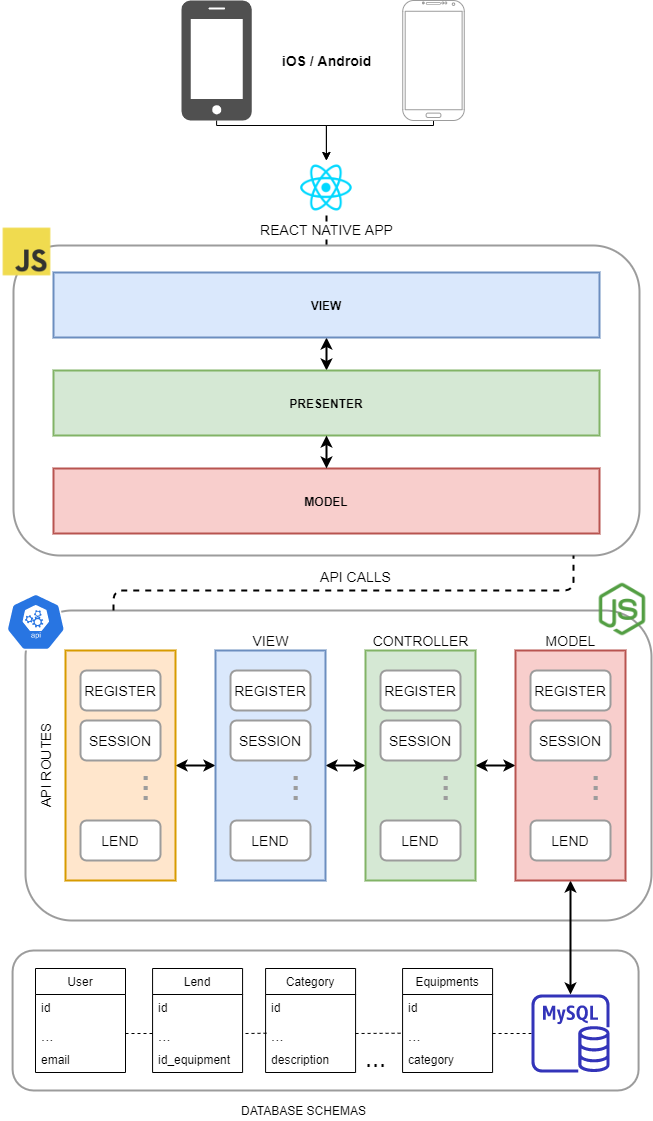
\includegraphics[width=9cm]{imagem/jubilant-octo-lab.png}
    \caption*{Fonte: Autor}
    \label{figura:lab-architecture}
    \end{figure}
    
    Após essas definições de arquitetura, citadas no paragráfo anterior, serão selecionadas as ferramentas e as principais bibliotecas disponibilizadas pelo JavaScript para compor o processo de desenvolvimento e a codificação do aplicativo, junto à escolha da estrutura de hierárquica de diretórios, configuração do ambiente de desenvolvimento e ambiente para os testes.
    
    A penúltima etapa consiste no desenvolvimento do aplicativo em si, considerando todos requisitos pré definidos e seguindo as especificações de interface elaborada na etapa de prototipagem e a escrita dos testes unitários e de integração para validar o comportamento do sistema perante o uso de suas funcionalidades, simulando objetos/usuários reais com metódos disponibilizados pelas bibliotecas que estão em uso na aplicação.
    
    E por fim, a implantação e disponibilização do aplicativo em Android e iOS, para alguns alunos e monitores da Universidade analisarem como o sistema se comporta em situações reais de empréstimo de equipamentos do laboratório. %Segue abaixo na tabela \ref{table:cronograma-tcc} o cronograma detalhado para o desenvolvimento do trabalho.
    
  %  \begin{table}[htb]
  %  \caption{Cronograma}
  %  \centering % para centralizarmos a figura
  %  \includegraphics[width=16cm]{imagem/cronograma-tcc.png}
  %  \caption*{Fonte: Autor}
  %  \label{table:cronograma-tcc}
  %  \end{table}
  
    \section{Plano de Testes}
    
    Visando a operabilidade do aplicativo, a escrita de testes automatizados de unidade e de integração que garantem a cobertura de todas as funcionalidades e ramificações/decisões do código para cercar toda a aplicação de possíveis efeitos colaterais durante o desenvolvimento, assegurando que as funcionalidades já implementadas continuam operando da maneira correta.
      
    \section{Homologação}
    
    Para garantir a aderência do aplicativo desenvolvido às necessidades dos usuários finais, foram realizados testes simulando situações reais de empréstimo e permitindo o primeiro contato dos usuários com o aplicativo. O objetivo desta etapa de homologação é avaliar sua usabilidade, junto as funcionalidades implementadas, validando se realmente atendem o propósito e se cumprem com os requisitos definidos anteriormente e se possível coletar melhorias que podem ser feitas para tornar o aplicativo ainda mais aderente ao processo.
